
%(BEGIN_QUESTION)
% Copyright 2013, Tony R. Kuphaldt, released under the Creative Commons Attribution License (v 1.0)
% This means you may do almost anything with this work of mine, so long as you give me proper credit

Most oscilloscopes can only directly measure voltage, not current.  One way to measure AC current with an oscilloscope is to measure the voltage dropped across a {\it shunt resistor}.  Since the voltage dropped across a resistor is proportional to the current through that resistor, whatever wave-shape the current is will be translated into a voltage drop with the exact same wave-shape.

However, one must be very careful when connecting an oscilloscope to any part of a grounded system, as many electric power systems are.  Note what happens here when a technician attempts to connect the oscilloscope across a shunt resistor located on the ``hot'' side of a grounded 120 VAC motor circuit:

$$\includegraphics[width=15.5cm]{i03474x01.eps}$$

Explain why sparks fly when an oscilloscope is connected to the AC circuit as shown.  Also, describe a safer way to perform this current measurement.

\underbar{file i03474}
%(END_QUESTION)





%(BEGIN_ANSWER)

Remember that an oscilloscope probe's reference clip is connected to the chassis of the oscilloscope, which in turn is connected to earth ground through the ground prong of the 120 VAC line power plug.  This means the ``hot'' side of the AC circuit under test is being shorted directly to earth ground through the oscilloscope!
 
\vskip 10pt

A better way to configure the oscilloscope to measure current is to set it up for {\it differential} measurement, where two channels and two probes are used, the oscilloscope's display set to show the difference between the two channels' signals.

\vskip 10pt

An entirely different approach would be to use a {\it current transformer} (CT) to sense current in the test circuit, with the CT's secondary current passing through a low-resistance shunt and one channel of the oscilloscope measuring that shunt resistor's voltage drop.  Here, grounding through the oscilloscope is not an issue because the current transformer provides galvanic isolation between the test circuit and the oscillscope.

%(END_ANSWER)





%(BEGIN_NOTES)


%INDEX% Electronics review: oscilloscope usage

%(END_NOTES)


